% =====================================================================
%  IN6049 --- Forecasting and Regression Analysis
%  Week 10: ARIMA Models and Exponential Smoothing --- Airline passengers
%
%  Built from template/slides-template.tex (Boadilla + seahorse, 16:9).
%  Title slide + 9 content slides.  Numbers come from Assigment_10.ipynb;
%  figures are its exported PNGs (images/ -> fig_*.png here).
%
%  Compiles on Overleaf with the default pdfLaTeX engine.
%  Upload alongside: fig_sim.png , fig_acfpacf.png , fig_resid.png ,
%  fig_arimafc.png , fig_compare.png
% =====================================================================
\documentclass[aspectratio=169,11pt]{beamer}

\usetheme{Boadilla}
\usecolortheme{seahorse}
\setbeamertemplate{navigation symbols}{}

\usepackage[utf8]{inputenc}
\usepackage[T1]{fontenc}
\usepackage{booktabs}
\usepackage{amsmath}
\usepackage{graphicx}
\usepackage{url}

% Emphasis lead-in: bold + structure colour.  Use as \key{Finding.} text...
\newcommand{\key}[1]{\textbf{\structure{#1}}}

% Figure placeholder, so the template compiles with no image files.
% Replace each use by  \includegraphics[width=0.9\linewidth]{@@ file @@}
% (vector PDF preferred; PNG is fine).
\newcommand{\figbox}[2]{%
  \fbox{\parbox[c][#2][c]{#1}{\centering\scriptsize\color{gray}@@ figure @@}}}

% ---------------------------------------------------------------------
\title[ARIMA and exponential smoothing]{ARIMA Models and Exponential Smoothing}
\subtitle{Monthly airline passengers, 1949--1960}
\author[Jie Dong, Elivier Reyes]{Jie Dong, Elivier Reyes}
\date[IN6049]{}

\begin{document}

% ===================== TITLE ========================================
\begin{frame}
  \titlepage
  \vspace{-1.2em}
  \begin{center}
    \small\urlstyle{same}\url{https://github.com/HelloJJJie/Assignment-Forecast-and-Analysis-of-Regression.git}

    \vspace{1.2em}
    Two ways to forecast the same series: a model of its own past
    (ARIMA) and a recursive weighted average (exponential smoothing).
  \end{center}
\end{frame}

% ===================== 1. AR, MA, ACF vs PACF =======================
\begin{frame}{1. AR, MA and the ACF/PACF signatures}
  \begin{columns}[T]
  \begin{column}{0.52\textwidth}
    \small
    $AR(p)$: $y_t=\phi_1y_{t-1}+\dots+\phi_py_{t-p}+\varepsilon_t$;
    $MA(q)$: $y_t=\varepsilon_t+\theta_1\varepsilon_{t-1}+\dots$;
    $\phi(B)(1-B)^dy_t=\delta+\theta(B)\varepsilon_t$ with
    $\theta(B)=1+\theta_1B+\dots$ (same plus sign in \texttt{statsmodels}).

    \vspace{0.3em}
    \key{ACF} $=$ total correlation at lag $k$; \key{PACF} $=$ direct
    correlation, the last coefficient of the regression of $y_t$ on
    $y_{t-1},\dots,y_{t-k}$ (checked: equals \texttt{statsmodels}).

    \vspace{0.3em}
    {\scriptsize\setlength{\tabcolsep}{3pt}
    \begin{tabular}{@{}lll@{}}
      \toprule
      Model & ACF & PACF \\
      \midrule
      $AR(p)$ & tails off & cuts off after $p$ \\
      $MA(q)$ & cuts off after $q$ & tails off \\
      $ARMA$  & tails off & tails off \\
      \bottomrule
    \end{tabular}}

    \vspace{0.3em}
    {\scriptsize Slide-6 examples: $AR(1)$, $\phi=0.7$: $\rho_k=0.70,0.49,0.34,0.24$;
    $MA(1)$, $\theta=0.5$: $\rho_1=0.40$, then $0$.}
  \end{column}
  \begin{column}{0.48\textwidth}
    \centering
    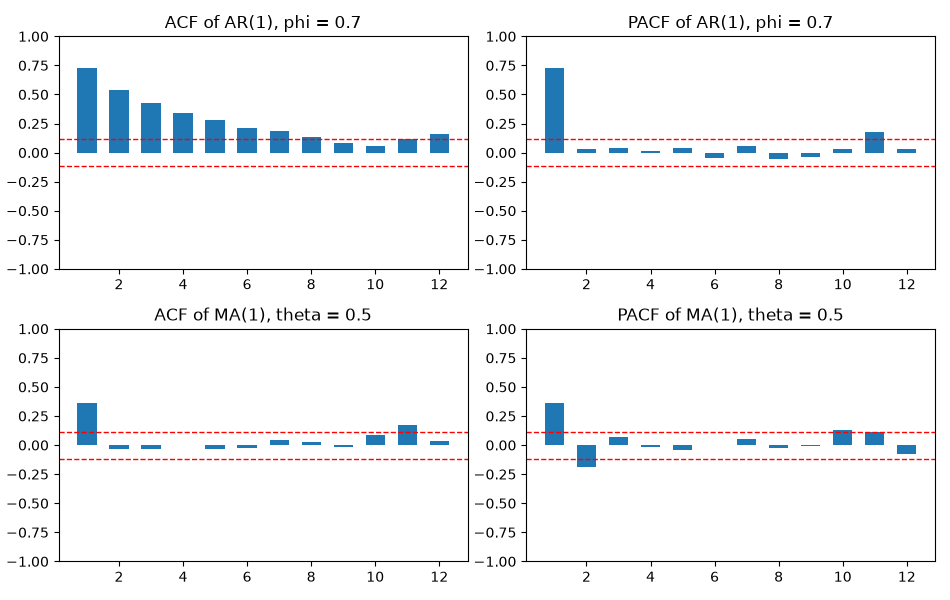
\includegraphics[width=0.96\linewidth]{fig_sim.png}

    \vspace{-0.1em}
    \raggedright\scriptsize
    Simulated $AR(1)$ and $MA(1)$ ($n=300$, bound $\pm0.115$). A few extra
    lags just beyond the bound (lag $11$, $12$, $10$) are chance exceedances:
    about $5\%$ of lags are expected to cross a $95\%$ bound.\par
  \end{column}
  \end{columns}
\end{frame}

% ===================== 2. IDENTIFICATION ON THE AIRLINE SERIES ======
\begin{frame}{2. Identification: making the series stationary, then reading the ACF and PACF}
  \begin{columns}[T]
  \begin{column}{0.46\textwidth}
    \small
    Non-constant variance $\Rightarrow$ log; trend $\Rightarrow$ regular
    difference $(1-B)$; yearly pattern $\Rightarrow$ seasonal difference
    $(1-B^{12})$. A slowly decaying ACF is the signal to difference
    (week 9: raw ACF above the bound at all $36$ lags). Training months $1$--$120$, $w_t=(1-B)(1-B^{12})\ln y_t$: $n=107$,
    $K=26$, bound $\pm0.193$.

    \vspace{0.2em}
    Beyond the bound (ACF / PACF): lag $1$ ($-0.33$ / $-0.33$), $3$ ($-0.22$ /
    $-0.21$), $12$ ($-0.41$ / $-0.37$), $23$ ($+0.23$ / $+0.20$); all others inside.

    \vspace{0.3em}
    \key{Reading:} spikes at lag $1$ and at the seasonal lag $12$ point to
    $MA(1)\times$seasonal $MA(1)_{12}$ --- the airline model. The PACF
    crosses at the same lags: no clean cut-off, so AR alternatives are fitted too.
  \end{column}
  \begin{column}{0.54\textwidth}
    \centering
    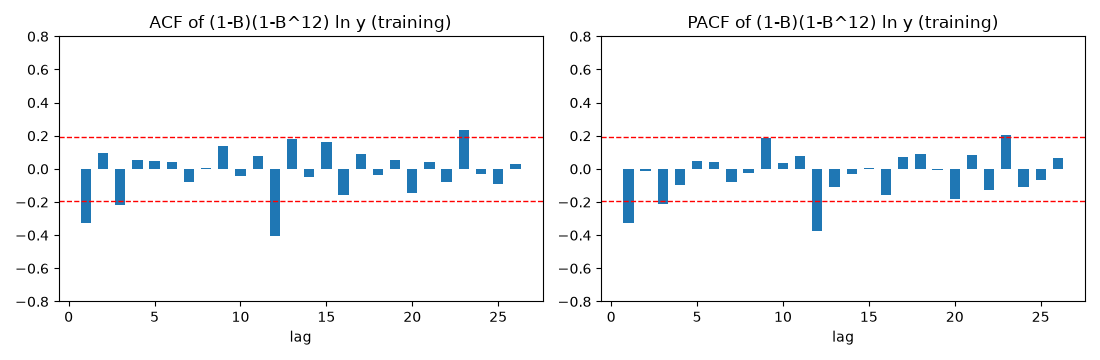
\includegraphics[width=0.98\linewidth]{fig_acfpacf.png}
  \end{column}
  \end{columns}
\end{frame}

% ===================== 3. ESTIMATION AND DIAGNOSTICS ================
\begin{frame}{3. Estimation and diagnostics: the Box--Jenkins loop}
  \begin{columns}[T]
  \begin{column}{0.56\textwidth}
    \small
    Candidates on $\ln y$, all $d=D=1$ (so AIC/BIC are comparable), maximum
    likelihood; Ljung--Box with $K=26$ and $K-k$ df ($k$ = fitted ARMA
    coefficients):

    \vspace{0.2em}
    {\scriptsize\setlength{\tabcolsep}{3pt}
    \begin{tabular}{@{}lrrrrr@{}}
      \toprule
      $SARIMA(p,1,q)(P,1,Q)_{12}$ & $k$ & $AIC$ & $BIC$ & $Q_{LB}$ & $P$ \\
      \midrule
      $(0,1,1)(0,1,1)$ & $2$ & $-389.01$ & $-380.99$ & $18.44$ & $0.78$ \\
      $(1,1,0)(0,1,1)$ & $2$ & $-388.64$ & $-380.62$ & $21.04$ & $0.64$ \\
      $(0,1,1)(1,1,0)$ & $2$ & $-384.23$ & $-376.21$ & $23.91$ & $0.47$ \\
      $(1,1,1)(0,1,1)$ & $3$ & $-387.28$ & $-376.59$ & $17.30$ & $0.79$ \\
      $(0,1,2)(0,1,1)$ & $3$ & $-387.07$ & $-376.37$ & $17.98$ & $0.76$ \\
      $(2,1,0)(0,1,1)$ & $3$ & $-386.66$ & $-375.97$ & $20.84$ & $0.59$ \\
      \bottomrule
    \end{tabular}}

    \vspace{0.3em}
    \small
    The airline model has the smallest AIC and BIC: $\hat\theta=-0.342$
    ($z=-3.9$), $\hat\Theta=-0.540$ ($z=-5.2$), $\hat\sigma^2=0.0014$. All
    candidates pass the residual check; the extra terms do not pay for
    themselves ($\Delta AIC\ge0.4$). AIC and BIC are the software's (they count
    $\sigma^2$, not divided by $T$): only differences matter.
  \end{column}
  \begin{column}{0.44\textwidth}
    \centering
    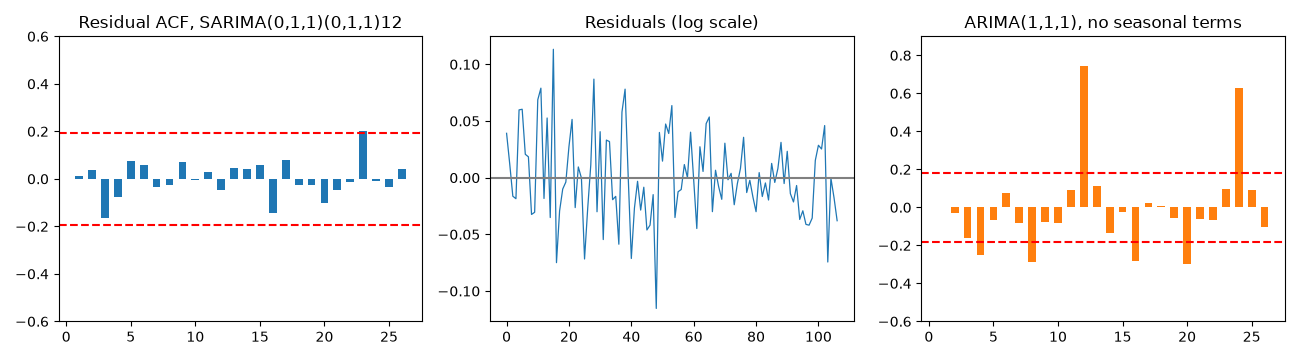
\includegraphics[width=0.98\linewidth]{fig_resid.png}

    \vspace{0.1em}
    \raggedright\scriptsize
    Left: residual ACF of the airline model (only lag $23$ marginally beyond
    the bound; normal probability plot $r=0.993$). Right: without the seasonal
    terms, ARIMA$(1,1,1)$ leaves $r_{12}=+0.74$ (bound $0.18$) and
    $Q_{LB}=201.8$, $P\approx10^{-28}$.\par
  \end{column}
  \end{columns}
\end{frame}

% ===================== 4. FORECASTING WITH ARIMA ====================
\begin{frame}{4. Forecasting with ARIMA: point forecasts and intervals}
  \begin{columns}[T]
  \begin{column}{0.48\textwidth}
    \small
    $\hat y_{t+h}=E[y_{t+h}\mid y_t,\dots]$; with $y_t=\sum_j\psi_j\varepsilon_{t-j}$,
    $\ \hat y_{t+h}\pm z_{\alpha/2}\sigma\sqrt{\sum_{j<h}\psi_j^2}$: the interval
    widens with $h$.

    \vspace{0.3em}
    \key{AR(1) example} ($\phi=0.7$, $\mu=50$, $y_t=58$, $\sigma=2$), slide 16:

    \vspace{0.2em}
    {\scriptsize
    \begin{tabular}{@{}rrrl@{}}
      \toprule
      $h$ & $\hat y_{t+h}$ & s.d. & $95\%$ interval \\
      \midrule
      $1$      & $55.6$ & $2.00$ & $(51.7,\,59.5)$ \\
      $2$      & $53.9$ & $2.44$ & $(49.1,\,58.7)$ \\
      $3$      & $52.7$ & $2.63$ & $(47.6,\,57.9)$ \\
      $\infty$ & $50.0$ & $2.80$ & $50\pm5.5$ \\
      \bottomrule
    \end{tabular}}

    \vspace{0.2em}
    {\tiny Slide shows $47.5$ for the $h=3$ lower limit ($52.7-5.2$); unrounded it is $47.57$.}

    \vspace{0.3em}
    \small
    \key{Airline model:} $\psi$-weights from the full operator
    $\phi(B)\Phi(B^{12})(1-B)(1-B^{12})$; the formula standard error equals the
    software's to $0.001\%$ ($0.0375$ at $h=1$, $0.155$ at $h=24$, log scale).
  \end{column}
  \begin{column}{0.52\textwidth}
    \centering
    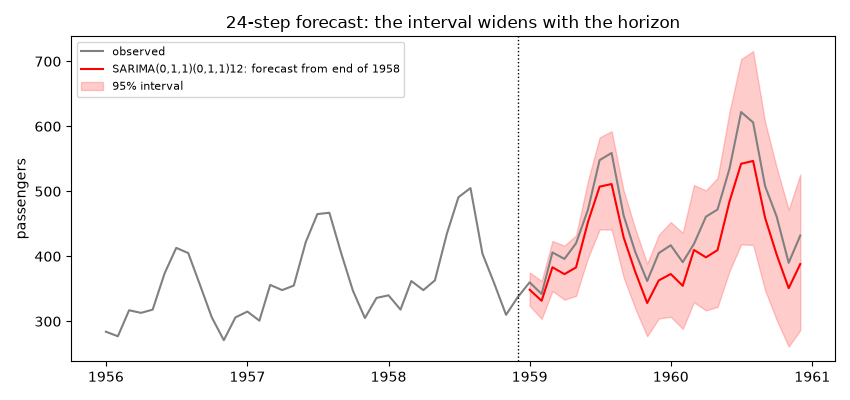
\includegraphics[width=0.98\linewidth]{fig_arimafc.png}

    \vspace{0.1em}
    \raggedright\scriptsize
    24 steps from the end of 1958: interval width $51$ ($h=1$), $129$ ($h=12$),
    $240$ ($h=24$); all $24$ actual values are inside. Point forecasts: MAPE
    $8.52\%$, RMSE $43.2$.\par
  \end{column}
  \end{columns}
\end{frame}

% ===================== 5. SIMPLE ES AND HOLT ========================
\begin{frame}{5. Exponential smoothing: simple and Holt}
  \begin{columns}[T]
  \begin{column}{0.50\textwidth}
    \small
    \key{Simple:} $\tilde y_t=\lambda y_t+(1-\lambda)\tilde y_{t-1}$, forecast
    $F_t=\tilde y_{t-1}$. Slide 5 ($\lambda=0.3$):

    \vspace{0.2em}
    {\scriptsize\setlength{\tabcolsep}{3pt}
    \begin{tabular}{@{}rrrr@{}}
      \toprule
      $t$ & $y_t$ & $F_t$ & $\tilde y_t$ \\
      \midrule
      $2$ & $135$ & $120.00$ & $124.50$ \\
      $4$ & $140$ & $124.65$ & $129.25$ \\
      $7$ & $160$ & $138.33$ & $144.83$ \\
      \bottomrule
    \end{tabular}}

    \vspace{0.1em}
    {\tiny Unrounded $129.255$, $138.335$; the slide rounds each step. $\hat y_8=144.83$.}

    \vspace{0.2em}
    \small
    \key{Holt:} $L_t=\alpha y_t+(1-\alpha)(L_{t-1}+T_{t-1})$,
    $T_t=\beta(L_t-L_{t-1})+(1-\beta)T_{t-1}$, $\hat y_{t+\tau}=L_t+\tau T_t$.
    Slide 9 ($\alpha=0.3$, $\beta=0.2$, $y=50,53,56,58$): $L_4=58.70$, $T_4=2.94$,
    $\hat y_5=61.64$, $\hat y_6=64.58$ (reproduced).
  \end{column}
  \begin{column}{0.50\textwidth}
    \small
    \key{On the airline series} (training months, constants by least squares):

    \vspace{0.2em}
    {\scriptsize
    \begin{tabular}{@{}lr@{}}
      \toprule
      simple: $\hat\lambda$            & $0.999$ \\
      Holt: $\hat\alpha,\ \hat\beta$   & $0.999,\ 0.006$ \\
      \bottomrule
    \end{tabular}}

    \vspace{0.3em}
    \begin{itemize}
      \item $\hat\lambda\to1$: the smoother becomes the naive forecast
            ($y_T$); one-step MAPE $9.73\%$, the same as naive.
      \item Holt adds a slope but no season: one-step MAPE $9.65\%$,
            24-step MAPE $14.5\%$.
      \item Neither can track a yearly cycle; simple smoothing lags the trend.
    \end{itemize}

    \vspace{0.2em}
    \small
    \key{Brown} double smoothing has \emph{one} constant $a$: Holt with
    $\alpha=a(2-a)$, $\beta=a/(2-a)$ (levels agree to $10^{-15}$).
  \end{column}
  \end{columns}
\end{frame}

% ===================== 6. HOLT-WINTERS ==============================
\begin{frame}{6. Holt--Winters: level, trend and season}
  \begin{columns}[T]
  \begin{column}{0.54\textwidth}
    \small
    \key{Additive:} $L_t=\alpha(y_t-S_{t-s})+(1-\alpha)(L_{t-1}+T_{t-1})$,
    $S_t=\gamma(y_t-L_t)+(1-\gamma)S_{t-s}$,
    $\hat y_{t+\tau}=L_t+\tau T_t+S_{t+\tau-s}$.
    \key{Multiplicative:} $y/S$ in $L_t$, $\gamma y_t/L_t$ in $S_t$,
    forecast $(L_t+\tau T_t)S_{t+\tau-s}$.

    \vspace{0.3em}
    Initial values: least squares on the first two seasons ($24$ months);
    constants minimise the one-step SSE ($t=13,\dots,120$):

    \vspace{0.2em}
    {\scriptsize\setlength{\tabcolsep}{3pt}
    \begin{tabular}{@{}lrrrr@{}}
      \toprule
       & $\hat\alpha$ & $\hat\beta$ & $\hat\gamma$ & SSE \\
      \midrule
      additive, $y$        & $0.240$ & $0.032$ & $0.999$ & $16{,}693$ \\
      multiplicative, $y$  & $0.310$ & $0.031$ & $0.999$ & $11{,}719$ \\
      additive, $\ln y$    & $0.373$ & $0.006$ & $0.838$ & $0.183$ (log) \\
      \bottomrule
    \end{tabular}}

    \vspace{0.2em}
    {\scriptsize $\hat\gamma\approx1$: the seasonal factors follow the latest year.
    The $\ln y$ row is on another scale: its SSE is not comparable.}
  \end{column}
  \begin{column}{0.46\textwidth}
    \small
    \key{Checked against \texttt{statsmodels}.}
    \begin{itemize}
      \item Additive: identical forecasts ($10^{-13}$). \texttt{statsmodels}
            writes $S_t=S_{t-s}+\gamma_{sm}e_t$; with $y_t-L_t=(1-\alpha)e_t$,
            $\gamma_{sm}=\gamma(1-\alpha)$.
      \item Multiplicative: \texttt{statsmodels} divides by the \emph{previous}
            level, the lecture by the new level $L_t$, so no constant maps one
            onto the other: they differ by $0.80$ on forecasts up to $478$;
            with \texttt{statsmodels}' own form the match is $10^{-13}$.
    \end{itemize}

    \vspace{0.3em}
    Initial multiplicative factors: Jan $0.889$, Jul $1.188$, Aug $1.180$,
    Nov $0.792$ (mean $1$).
  \end{column}
  \end{columns}
\end{frame}

% ===================== 7. LINK TO ARIMA =============================
\begin{frame}{7. The link to ARIMA: when is a smoother an ARIMA model?}
  \begin{columns}[T]
  \begin{column}{0.54\textwidth}
    \small
    Simple smoothing $\equiv$ ARIMA$(0,1,1)$ with $\lambda=1+\theta_1$
    (lecture sign: $\theta_1=-(1-\lambda)$); Holt $\equiv$ ARIMA$(0,2,2)$ with
    $\theta_1=\alpha+\alpha\beta-2$, $\theta_2=1-\alpha$. Shown on two
    \emph{synthetic} series where the smoother is the right model:

    \vspace{0.3em}
    \begin{itemize}
      \item \key{Local level:} ARIMA$(0,1,1)$ gives $\hat\theta_1=-0.603$, so
            $\lambda=0.397$ (theory $0.390$; the least-squares smoother gives
            $0.397$); one-step forecasts differ by $1.4\times10^{-5}$.
      \item \key{Local linear trend:} ARIMA$(0,2,2)$ gives
            $\hat\theta=(-1.662,\,+0.695)$, so $\alpha=0.305$, $\beta=0.109$.
            The forecasts start from different initial states and the gap falls
            from $0.25$ ($t>20$) to $10^{-7}$ ($t>100$): the same predictor in
            the limit.
    \end{itemize}
  \end{column}
  \begin{column}{0.46\textwidth}
    \small
    \key{The airline series is not such a series.} On $\ln y$:
    \begin{itemize}
      \item ARIMA$(0,1,1)$: $\hat\theta_1=+0.277$, so $\lambda=1.277$, outside
            $(0,1)$ --- not a simple smoother.
      \item ARIMA$(0,2,2)$: $\alpha=1.279$, $\beta=0.001$ --- not a Holt
            smoother.
    \end{itemize}
    The season is what these models cannot express; Holt--Winters and
    SARIMA add it.

    \vspace{0.3em}
    \key{Sign convention.} The lecture and \texttt{statsmodels} both use
    $\theta(B)=1+\theta_1B$; sources that write $1-\theta_1B$ flip the sign.
  \end{column}
  \end{columns}
\end{frame}

% ===================== 8. HOLD-OUT COMPARISON =======================
\begin{frame}{8. Hold-out comparison: the last $24$ months}
  \begin{columns}[T]
  \begin{column}{0.58\textwidth}
    \small
    Models fitted on $1949$--$1958$. $24$-step: forecasts from the end of
    $1958$; one-step: constants fixed, the state keeps updating.

    \vspace{0.2em}
    {\scriptsize\setlength{\tabcolsep}{3pt}
    \begin{tabular}{@{}lrrrr@{}}
      \toprule
       & \multicolumn{2}{c}{$24$-step} & \multicolumn{2}{c}{one-step} \\
       & MAPE \% & RMSE & MAPE \% & RMSE \\
      \midrule
      simple smoothing                 & $23.58$ & $137.4$ & $9.73$ & $51.8$ \\
      Holt                             & $14.52$ & $97.4$  & $9.65$ & $51.8$ \\
      Holt--Winters additive, $y$      & $6.69$  & $35.8$  & $2.68$ & $15.0$ \\
      Holt--Winters multiplicative, $y$ & $7.30$ & $36.8$  & $2.59$ & $14.9$ \\
      Holt--Winters additive, $\ln y$  & $3.85$  & $19.1$  & $2.29$ & $14.6$ \\
      SARIMA$(0,1,1)(0,1,1)_{12}$      & $8.52$  & $43.2$  & $2.55$ & $15.3$ \\
      \bottomrule
    \end{tabular}}

    \vspace{0.3em}
    \small
    Week 9, trend + season + AR(1), refitted each month: one-step MAPE $3.56\%$.
  \end{column}
  \begin{column}{0.42\textwidth}
    \centering
    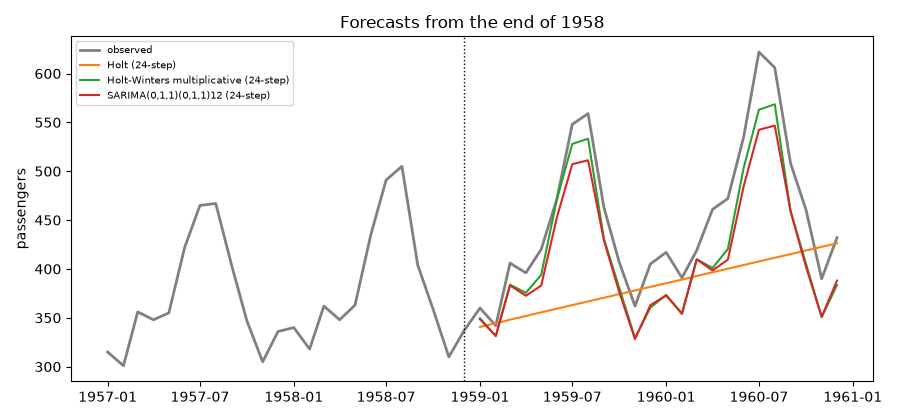
\includegraphics[width=0.98\linewidth]{fig_compare.png}

    \vspace{0.1em}
    \raggedright\scriptsize
    Without a season (Holt) the forecast misses the yearly cycle. SARIMA and
    multiplicative Holt--Winters follow it but under-forecast the 1960 peaks.\par
  \end{column}
  \end{columns}
\end{frame}

% ===================== 9. SUMMARY ===================================
\begin{frame}{9. Which method for which series? Summary}
  \small
  \begin{itemize}
    \item \key{ARIMA:} difference until the ACF stops decaying, read ACF/PACF,
          fit, check the residuals, compare AIC/BIC. Here: log, $(1-B)(1-B^{12})$
          and two MA terms; Ljung--Box $P=0.78$; the $95\%$ intervals widen with
          $h$ and cover all $24$ held-out months.
    \item \key{Exponential smoothing:} simple (level), Holt (+ trend),
          Holt--Winters (+ season). Only Holt--Winters follows this series:
          one-step MAPE $2.3$--$2.7\%$ against $9.7\%$ for simple smoothing and Holt.
    \item \key{They overlap:} simple smoothing is ARIMA$(0,1,1)$ and Holt is
          ARIMA$(0,2,2)$ on that kind of series; seasonal data need seasonal terms.
  \end{itemize}

  \vspace{0.1em}
  {\scriptsize\setlength{\tabcolsep}{3pt}
  \begin{tabular}{@{}lll@{}}
    \toprule
    Series has & Method & Forecast \\
    \midrule
    level only            & simple smoothing & $\tilde y_T$ (flat) \\
    level + trend         & Holt             & $L_T+\tau T_T$ \\
    level + trend + season & Holt--Winters   & $L_T+\tau T_T+S_{T+\tau-s}$ \\
    own past + shocks      & (S)ARIMA        & conditional expectation, interval $\pm z\sigma\sqrt{\sum\psi_j^2}$ \\
    \bottomrule
  \end{tabular}}

  \vspace{0.2em}
  \small
  \key{Takeaway.} Here the best simple recipe is Holt--Winters on $\ln y$
  ($3.85\%$ over $24$ steps); SARIMA is the one with a formal error check and an interval.
\end{frame}

\end{document}
